% \documentclass[handout]{beamer}
\documentclass{beamer}

\mode<presentation>
{
  \usetheme{ANLBlue}
  % \usefonttheme[onlymath]{serif}
  % \usetheme{Singapore}
  % \usetheme{Warsaw}
  % \usetheme{Malmoe}
  % \useinnertheme{circles}
  % \useoutertheme{infolines}
  % \useinnertheme{rounded}

  \setbeamercovered{transparent=20}
}

\usepackage[english]{babel}
\usepackage[latin1]{inputenc}
\usepackage{alltt,listings,multirow,ulem,siunitx}
\usepackage[absolute,overlay]{textpos}
\TPGrid{1}{1}
\usepackage{pdfpages}
\usepackage{ulem}
\usepackage{multimedia}
\usepackage{multicol}
\newcommand\hmmax{0}
\newcommand\bmmax{0}
\usepackage{bm}
\usepackage{comment}
\usepackage{subcaption}

% font definitions, try \usepackage{ae} instead of the following
% three lines if you don't like this look
\usepackage{mathptmx}
\usepackage[scaled=.90]{helvet}
% \usepackage{courier}
\usepackage[T1]{fontenc}
\usepackage{tikz}
\usetikzlibrary{decorations.pathreplacing}
\usetikzlibrary{shadows,arrows,shapes.misc,shapes.arrows,shapes.multipart,arrows,decorations.pathmorphing,backgrounds,positioning,fit,petri,calc,shadows,chains,matrix}

\newcommand\vvec{\bm v}
\newcommand\bvec{\bm b}
\newcommand\bxk{\bvec_0 \times \kappa_0 \cdot \nabla}
\newcommand\delp{\nabla_\perp}

% \usepackage{pgfpages}
% \pgfpagesuselayout{4 on 1}[a4paper,landscape,border shrink=5mm]

\usepackage{JedMacros}

\newcommand{\timeR}{t_{\mathrm{R}}}
\newcommand{\timeW}{t_{\mathrm{W}}}
\newcommand{\mglevel}{\ensuremath{\ell}}
\newcommand{\mglevelcp}{\ensuremath{\mglevel_{\mathrm{cp}}}}
\newcommand{\mglevelcoarse}{\ensuremath{\mglevel_{\mathrm{coarse}}}}
\newcommand{\mglevelfine}{\ensuremath{\mglevel_{\mathrm{fine}}}}

%solution and residual
\newcommand{\vx}{\ensuremath{x}}
\newcommand{\vc}{\ensuremath{\hat{x}}}
\newcommand{\vr}{\ensuremath{r}}
\newcommand{\vb}{\ensuremath{b}}

%operators
\newcommand{\vA}{\ensuremath{A}}
\newcommand{\vP}{\ensuremath{I_H^h}}
\newcommand{\vS}{\ensuremath{S}}
\newcommand{\vR}{\ensuremath{I_h^H}}
\newcommand{\vI}{\ensuremath{\hat I_h^H}}
\newcommand{\vV}{\ensuremath{\mathbf{V}}}
\newcommand{\vF}{\ensuremath{F}}
\newcommand{\vtau}{\ensuremath{\mathbf{\tau}}}


\title{Tutorial on Git}
\subtitle{Distributed Version Control and Development Workflow}
\author{{\bf Jed Brown} \texttt{jedbrown@mcs.anl.gov} \\
\quad Thanks to Doug Jacobsen, Jeff Johnson, James Foucar, Susannah Burrows, Rob Jacob, Andy Salinger}

% - Use the \inst command only if there are several affiliations.
% - Keep it simple, no one is interested in your street address.
% \institute
% {
%   Mathematics and Computer Science Division \\ Argonne National Laboratory
% }

\date{ACME All-Hands Meeting, 2015-05-06 \\[1em]
This talk: \url{http://59A2.org/files/20150506-GitTutorial.pdf}}

% This is only inserted into the PDF information catalog. Can be left
% out.
\subject{Talks}


% If you have a file called "university-logo-filename.xxx", where xxx
% is a graphic format that can be processed by latex or pdflatex,
% resp., then you can add a logo as follows:

% \pgfdeclareimage[height=0.5cm]{university-logo}{university-logo-filename}
% \logo{\pgfuseimage{university-logo}}



% Delete this, if you do not want the table of contents to pop up at
% the beginning of each subsection:
% \AtBeginSubsection[]
% {
% \begin{frame}<beamer>
%   \frametitle{Outline}
%   \tableofcontents[currentsection,currentsubsection]
% \end{frame}
% }

% \AtBeginSection[]
% {
%   \begin{frame}<beamer>
%     \frametitle{Outline}
%     \tableofcontents[currentsection]
%   \end{frame}
% }

% If you wish to uncover everything in a step-wise fashion, uncomment
% the following command:

% \beamerdefaultoverlayspecification{<+->}

\begin{document}
\lstset{language=C}
\normalem

\begin{frame}
  \titlepage
\end{frame}

\begin{frame}{Distributed Version Control}
  \begin{itemize}
  \item Directed Acyclic Graph (DAG) history
    \begin{itemize}
    \item Every commit has one or more ancestors
    \item Labels and namespaces
    \item Branch structure to organize workflow
    \item Flexible, asynchronous reviewing and quality control
    \item Powerful merging
    \end{itemize}
  \item Work with clones, each is equivalent and fully-functional
    \begin{itemize}
    \item Social conventions for which (if any) is canonical
    \item Each has its own branch namespace
    \end{itemize}
  \item Provenance and auditability via cryptographic hashes
  \item Operations are local (and fast)
  \end{itemize}
\end{frame}

\begin{frame}{Is linear history good?}
  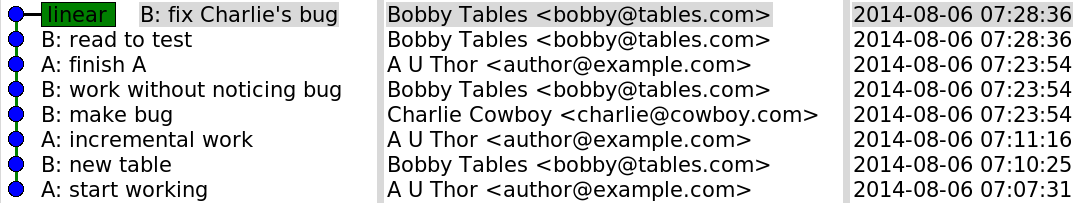
\includegraphics[width=\textwidth]{figures/Git/history-linear.png}
  \begin{itemize}
  \item Testing and review?  Bugs and fixes are spread out.
  \item When is a feature complete?
  \end{itemize}
  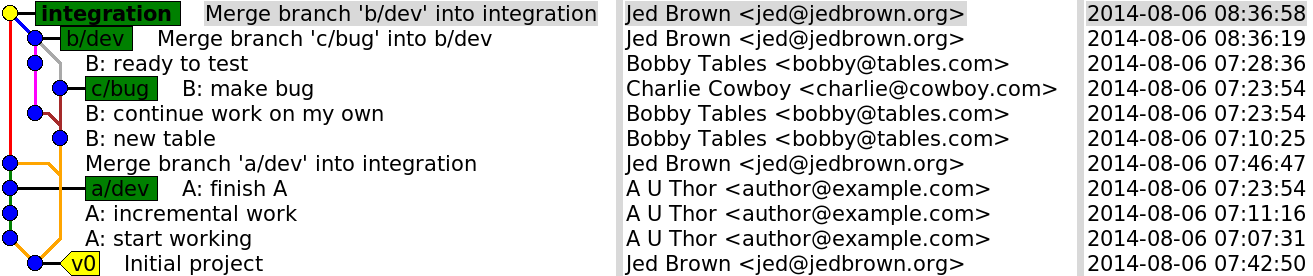
\includegraphics[width=\textwidth]{figures/Git/history-branch.png}
  \begin{itemize}
  \item Merges contain completed features.
  \item Asynchronous testing and review.
  \end{itemize}
  {\small Output from \texttt{gitk}}
\end{frame}

\begin{frame}{Labeling the DAG}
  \begin{columns}
    \begin{column}{0.5\textwidth}
      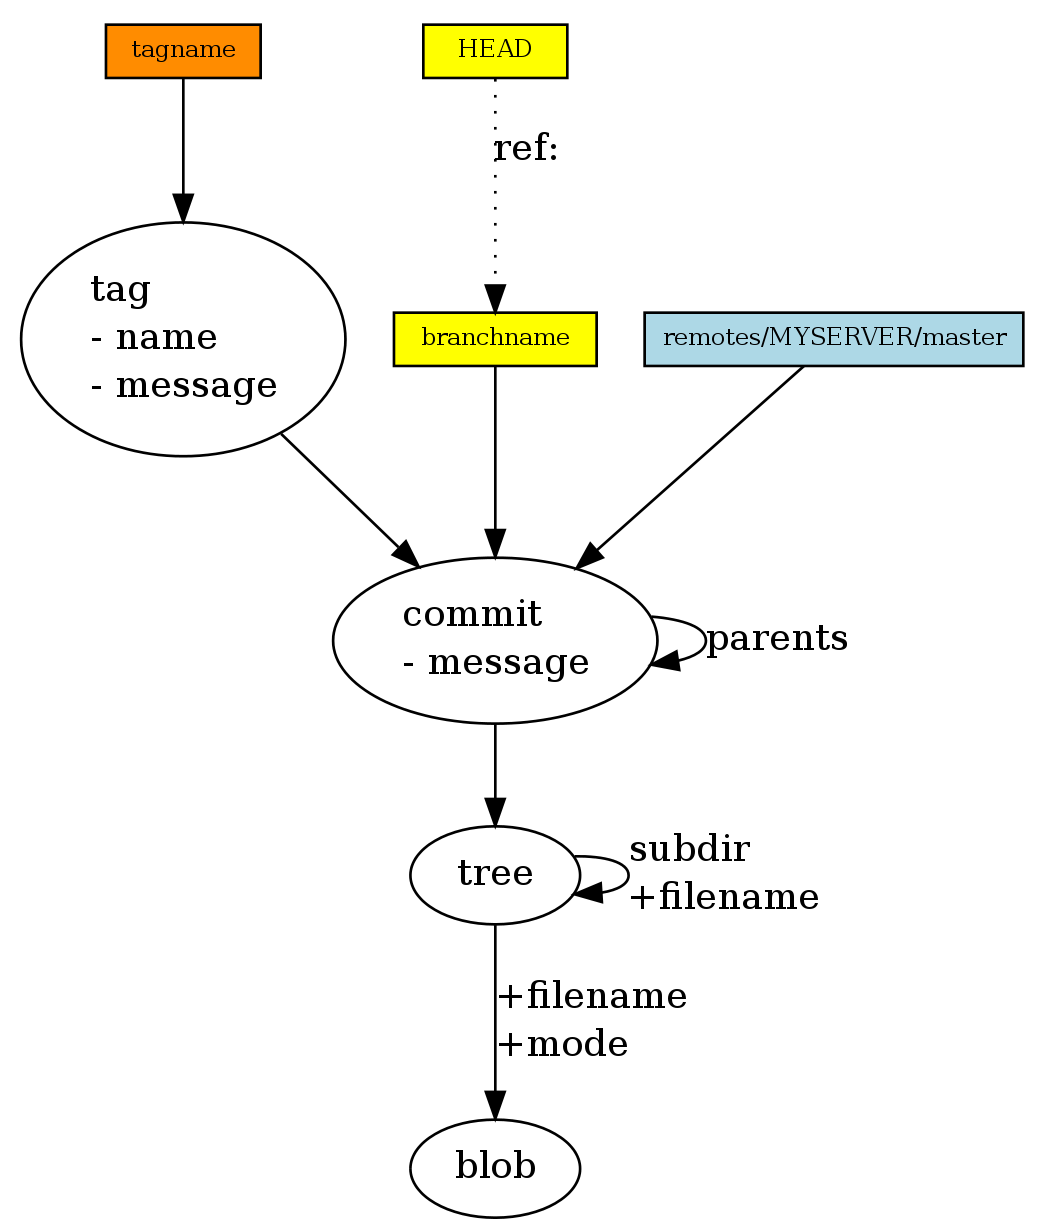
\includegraphics[width=\textwidth]{figures/Git/git-storage.png} \\
    \end{column}
    \begin{column}{0.5\textwidth}
      \begin{itemize}
      \item {\tt HEAD}: cursor naming ``current branch'' or tag/commit
        \begin{itemize}
        \item If a branch (usually), committing will advance that branch
        \item Implicit reference for many commands (like \texttt{git diff})
        \end{itemize}
      \item Branches: lightweight labels that move with cursor (HEAD) and push/pull
      \item Tags: stationary, can be signed
      \item Hashes: every object is uniquely identifiable by a SHA1 hash
      \end{itemize}
    \end{column}
  \end{columns}
  {\tiny \url{http://eagain.net/articles/git-for-computer-scientists/}}
\end{frame}

\begin{frame}{Basic DAG commands}
  \textbf{Git is fundamentally a tool for incrementally updating and analyzing the labeled DAG.}
  \begin{tabular}{l p{2.8in}}
    \toprule
    \texttt{commit} & create a new node in DAG and advance HEAD \\
    \texttt{checkout} \textit{name} & move HEAD to specified branch and update working tree to match \\
    \texttt{branch} \textit{name} & create new branch label \\
    \texttt{tag} \textit{name} & create (stationary) tag on commit indicated by HEAD \\
    \texttt{merge} \textit{commitish} & merge specified branch/tag/commit into current branch, creating new commit and advancing HEAD \\
    \midrule
    \texttt{log} & ancestors of HEAD \\
    \texttt{log -{}-first-parent} & ancestors of HEAD following only first parent of merges \\
    \texttt{log -{}-} \textit{path} & only those that modify path \\
    \bottomrule
  \end{tabular}
\end{frame}

\begin{frame}{Hands-on: configuration}
  \begin{itemize}
  \item \texttt{git config -{}-global user.name 'Your Name'}
  \item \texttt{git config -{}-global user.email your.name@lab.gov}
  \item \texttt{git config -{}-global push.default nothing}
  \item \texttt{git config -{}-global color.ui auto}
  \item Optional: \url{https://raw.githubusercontent.com/git/git/master/contrib/completion/git-prompt.sh}
  \item Optional: \url{https://raw.github.com/git/git/master/contrib/completion/git-completion.bash}
  \item \texttt{git config -{}-global merge.log true}
  \item \url{https://acme-climate.atlassian.net/wiki/display/Docs/Development+Quick+Guide}
  \end{itemize}
\end{frame}

\begin{frame}{Hands-on: clone a repository}
  \begin{itemize}
  \item \texttt{git clone git@github.com:ACME-Climate/git-tutorial} \\
    {\small or \texttt{https://YourName@github.com/ACME-Climate/git-tutorial}}
  \item \texttt{cd git-tutorial}
  \item Compare the history
    \begin{itemize}
    \item \texttt{git log -{}-graph}
    \item \texttt{git checkout linear \&\& git log -{}-graph}
    \item \texttt{git checkout integration \&\& git log origin/a/dev..}
    \end{itemize}
  \end{itemize}
  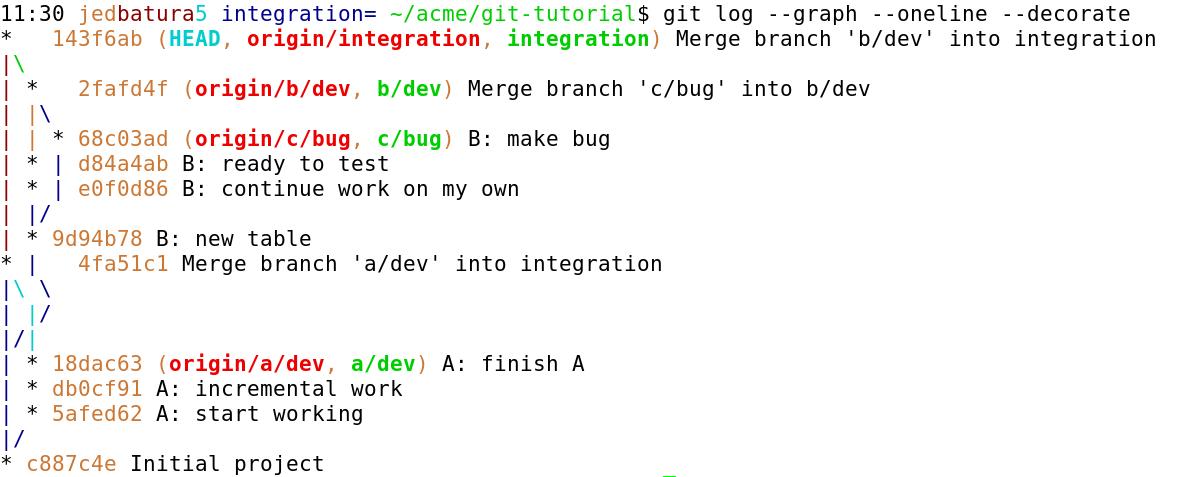
\includegraphics[width=\textwidth]{figures/Git/log-graph-integration.png} \\
\end{frame}

\begin{frame}{The staging area (or ``index'')}
  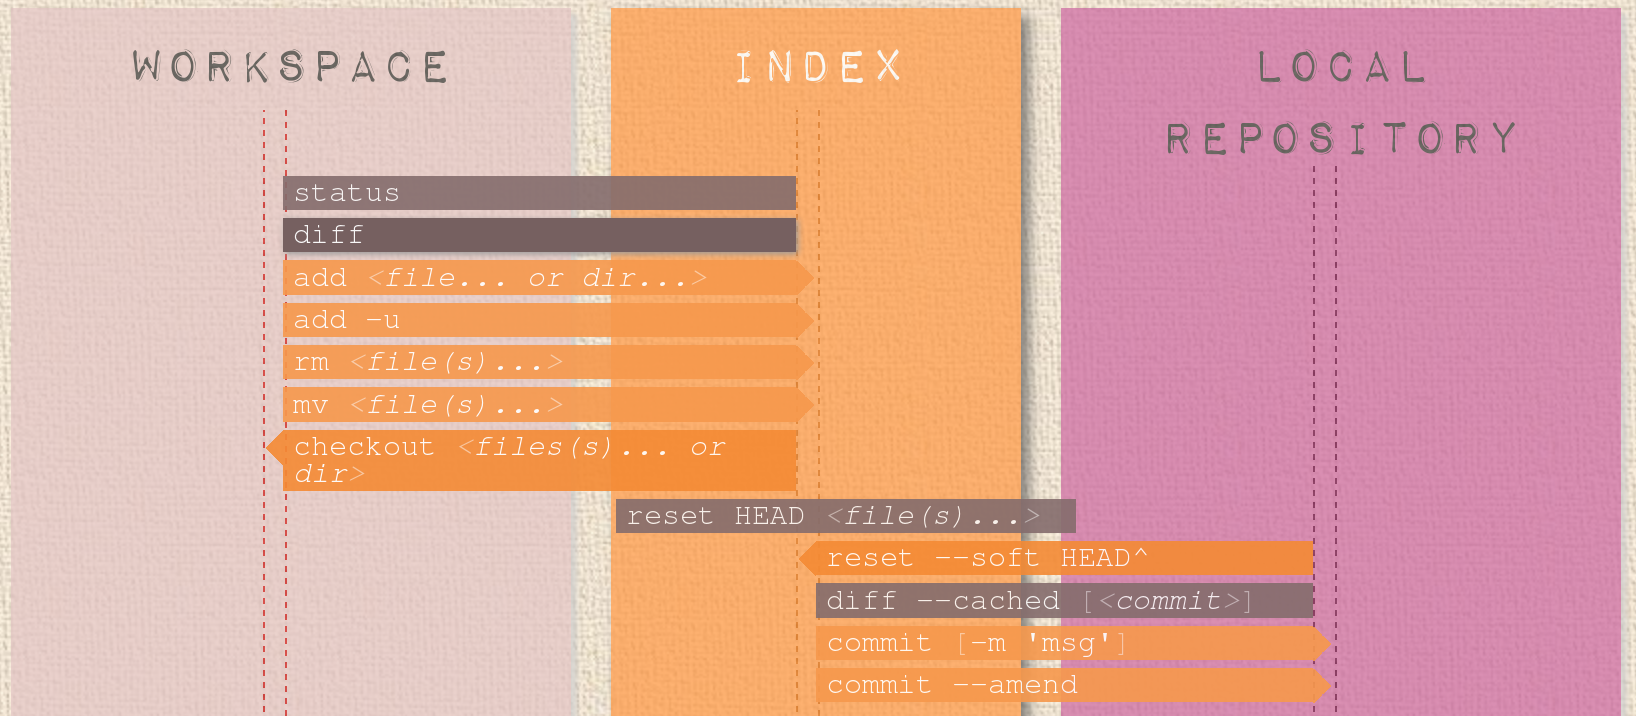
\includegraphics[width=\textwidth]{figures/Git/staging-area.png} \\
  {\tiny \url{http://ndpsoftware.com/git-cheatsheet.html}}
  \begin{itemize}
  \item Sometimes we don't want to commit everything
  \item It's nice to incrementally resolve conflicts, then not be shown again
  \item \texttt{git add}, \texttt{git rm}, and others need to be logged somehow
  \item Fast and useful primitive for building tools (in Git and externally)
  \end{itemize}
\end{frame}

\begin{frame}{Remotes}
  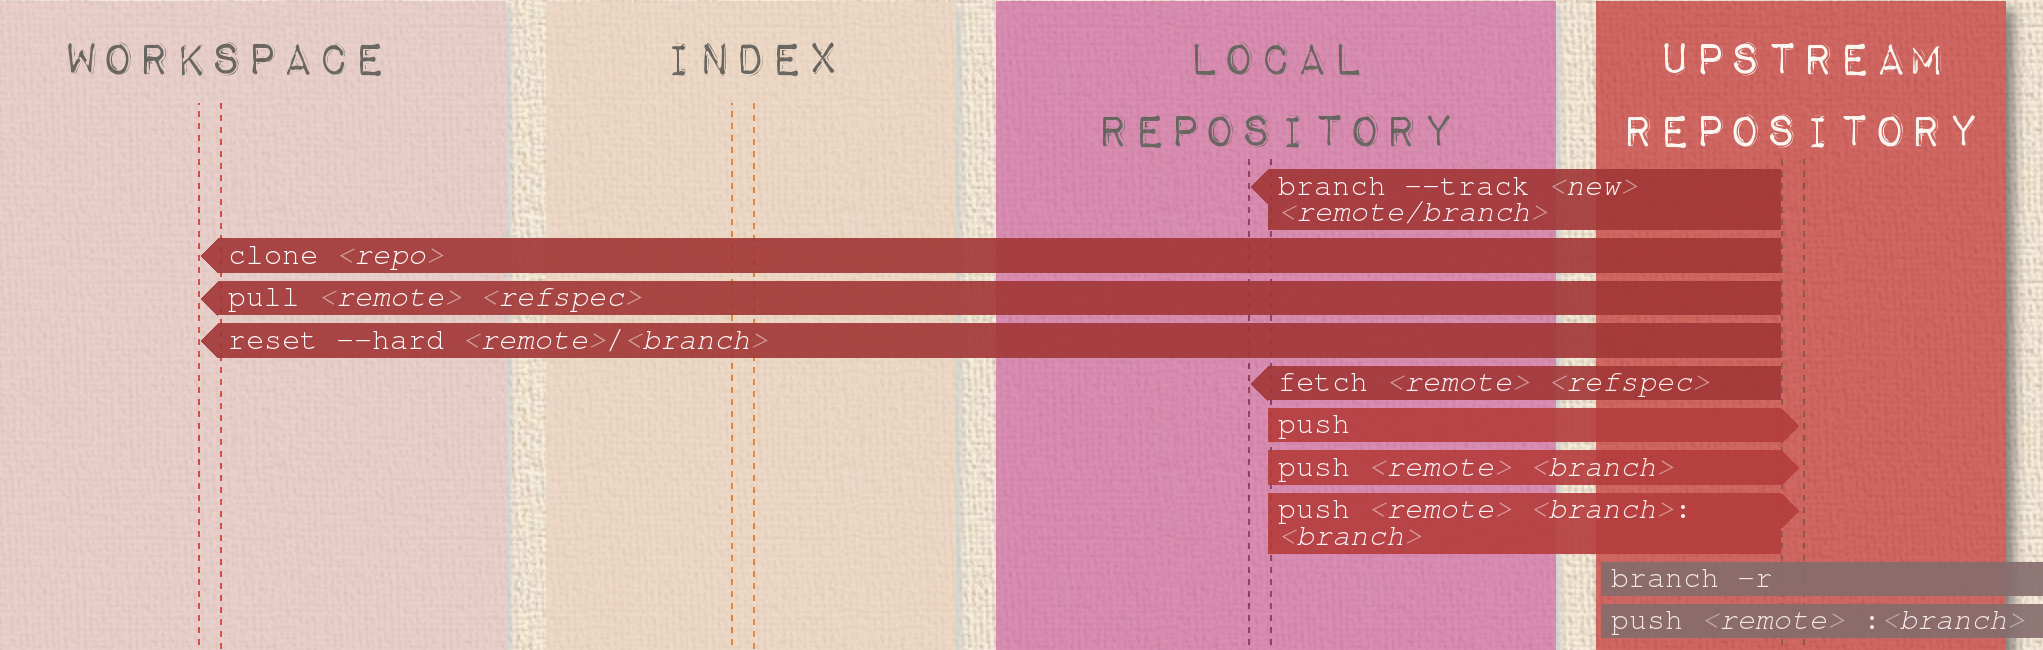
\includegraphics[width=\textwidth]{figures/Git/remote-repo.png} \\
  \begin{itemize}
  \item Remotes are named and cached remote repositories
    \begin{itemize}
    \item more commands can complete locally
    \end{itemize}
  \item Cache is updated by \texttt{git fetch} and similar
  \item Private namespace for branches (prevents conflicts)
  \item ``origin'' is created by default by \texttt{git clone}
  % \item \texttt{git remote add origin git@github.com:ACME-Climate/git-tutorial}
  \end{itemize}
\end{frame}

\begin{frame}{Hands-on: make a commit to show you were here}
  \begin{itemize}
  \item \texttt{git checkout attendees}
  \item \texttt{git checkout -b jed/attendee}
  \item \texttt{echo 'Argonne  SEG' > Jed\_Brown}
  \item \texttt{git add Jed\_Brown}
  \item \texttt{git commit -m"I'm at the Git tutorial"}
  \item Submit changes
    \begin{itemize}
    \item \texttt{git push -u origin jed/attendee} \\
    \end{itemize}
  \item Turn to your neighbor and rock-paper-scissors to elect an integrator.
    \begin{itemize}
    \item Integrator: review your neighbor's branch
    \item \texttt{git fetch \&\& git checkout neighbor/attendee \&\& git log -p}
    \item If it looks good: \texttt{git checkout me/attendee \&\& git merge neighbor/attendee \&\& git push}
    \item Make a pull request to 'attendees' at \url{https://github.com/ACME-Climate/git-tutorial}
    \end{itemize}
  \end{itemize}
\end{frame}

\begin{frame}{Working with branches}
  In your browser: \url{https://pcottle.github.io/learnGitBranching/}
  \begin{itemize}
  \item Spend a few minutes with the branching and merging examples
  \item Advanced commands
  \end{itemize}
  \begin{tabular}{l p{2.8in}}
    \toprule
    \texttt{reset} \textit{path} & set staging area to match \textit{path} in HEAD \\
    \texttt{rebase} \textit{commit} & replay commits in \texttt{\$\{commit\}..} on top of \texttt{\$\{commit\}}, advancing current branch (old commits will be gc'd if not referenced) \\
    \texttt{rebase -{}-abort} & go back to state before starting rebase \\
    \texttt{rebase -i HEAD\~{}3} & interactively amend last three commits \\
    \texttt{cherry-pick} \textit{commit} & make commit on current branch, effecting the same change as \texttt{\$\{commit\}} \\
    \midrule
    \texttt{reflog} & everywhere that HEAD has been in last 90 days (good to recover after a mistake) \\
    \texttt{gitk} & graphical history visualization \\
    \texttt{git citool} & graphical incremental commit tool \\
    \bottomrule
  \end{tabular}  
\end{frame}

% git init linear
% echo 1 > a
% git add a
% git commit --author='A U Thor <author@example.com>' -m'A: start working'
% echo 1 > b
% git add b
% git commit --author='Bobby Tables <bobby@tables.com>' -m'B: new table'
% echo 2 >> a
% git commit --author='A U Thor <author@example.com>' -m'A: incremental work' -a
% echo 0 >> b
% git commit --author='Charlie Cowboy <charlie@cowboy.com>' -m'B: make bug' -a
% echo 2 >> b
% git commit --author='Bobby Tables <bobby@tables.com>' -m'B: work without noticing bug' -a
% echo 3 >> a
% git commit --author='A U Thor <author@example.com>' -m'A: finish A' -a
% echo 3 >> b
% git commit --author='Bobby Tables <bobby@tables.com>' -m'B: ready to test' -a
% sed s/0/4/ b | sort > tmp; mv tmp b
% git commit --author='Bobby Tables <bobby@tables.com>' -m"B: fix Charlie's bug" -a



\section{Development Workflow}
\begin{frame}{Git Workflow Objectives}
  \begin{itemize}
  \item 'master' is always stable and ready to release
  \item features are complete and tested before appearing in 'master'
  \item commits are minimal logically coherent, reviewable, and testable units
  \item related commits go together so as to be reviewable and debuggable by specialist
  \item new development is not disrupted by others' features and bugs
  \item rapid collaboration between developers possible
  \item \texttt{git log -{}-first-parent maint..master} reads like a changelog
  \item bugs can be fixed once and anyone that needs the fix can obtain it without side-effects
  \end{itemize}
\end{frame}

\begin{frame}{Simplified gitworkflows(7)}
  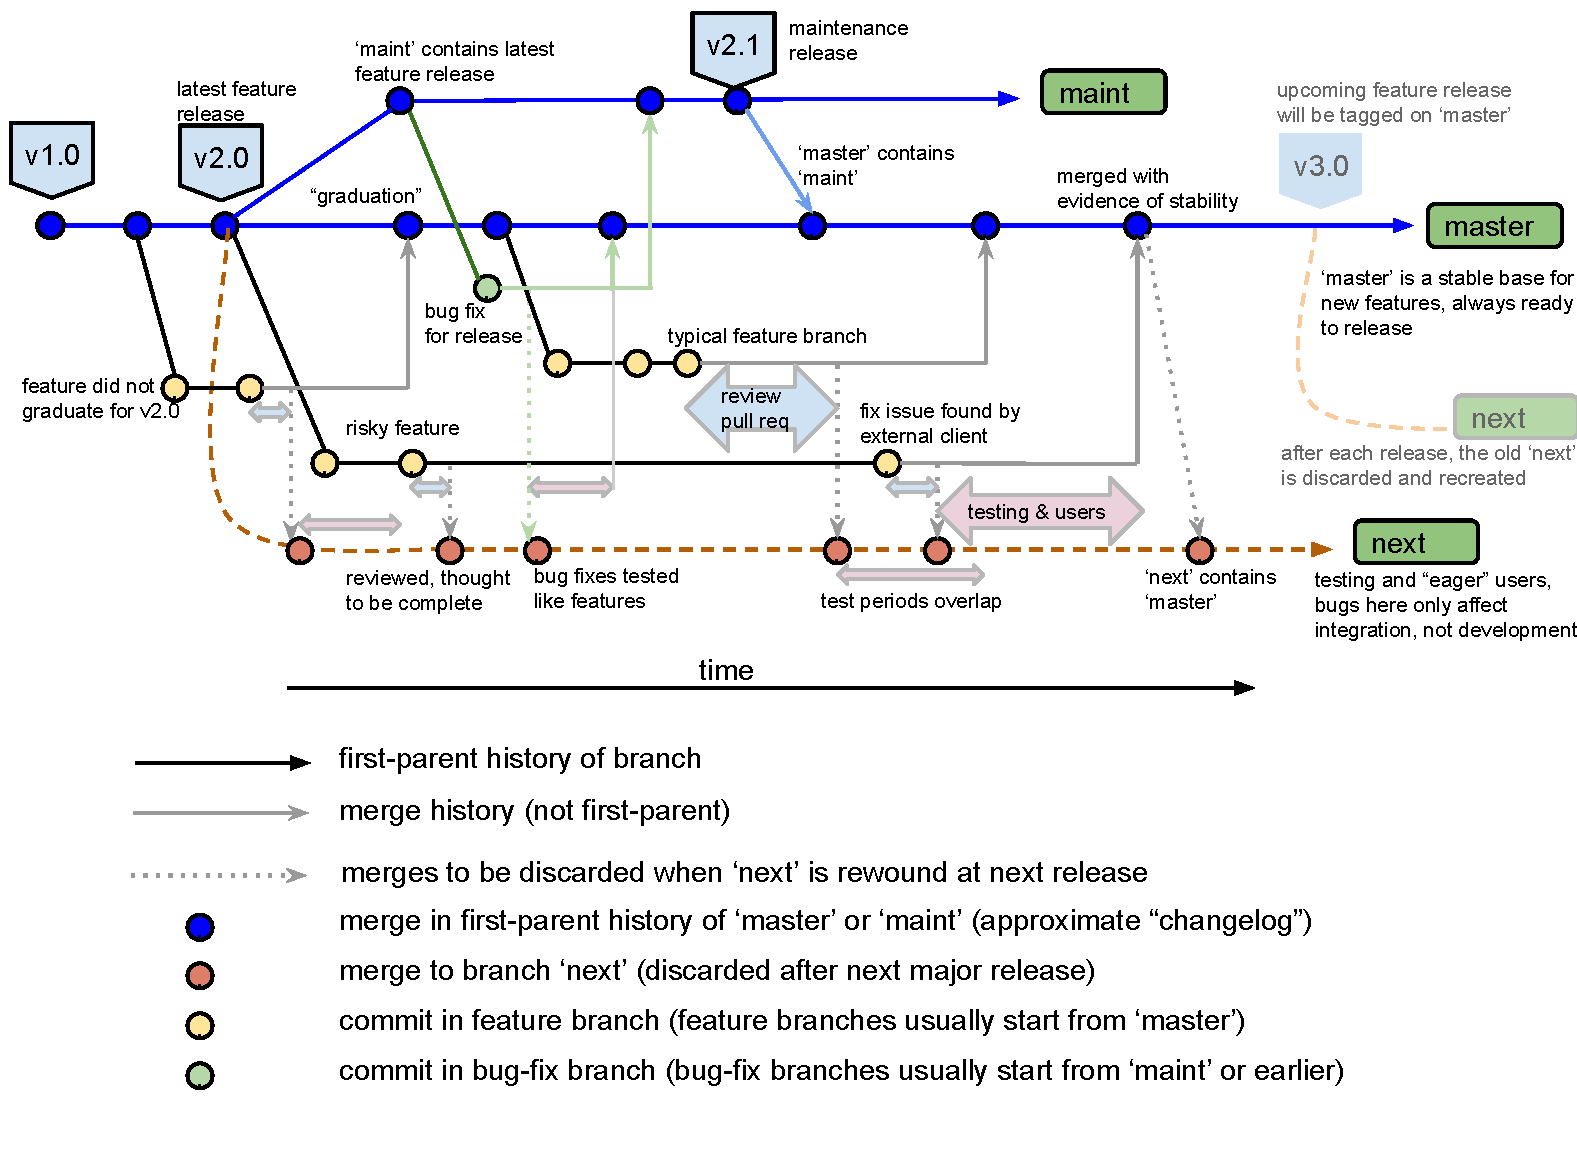
\includegraphics[width=\textwidth]{figures/Git/simplified-gitworkflows7.pdf}
\end{frame}

\begin{frame}{ACME Best Practices}
  \begin{itemize}
  \item Every branch has a purpose
  \item Distinguish integration branches from topic branches
  \item Do all development in topic branches
    \begin{itemize}
    \item \texttt{git checkout -b my/component/short-feature-description master}
    \end{itemize}
  \item \href{https://acme-climate.atlassian.net/wiki/display/Docs/Branch\%2C+Tag\%2C+and+Version+name+conventions}{Namespace your branches}
  \item Write clear commit messages for reviewers and people trying to debug your code
  \item \href{https://bitbucket.org/petsc/petsc/wiki/developer-instructions-git\#markdown-header-merging}{Avoid excessive merging from upstream}
    \begin{itemize}
    \item Always write a clear commit message explaining what is being merged and why
    \end{itemize}
  \end{itemize}
  {\bf Integrators}
  \begin{itemize}
  \item Merge integration branches ``forward''
    \begin{itemize}
    \item \texttt{maint} $\to$ \texttt{master} $\to$ \texttt{next}
    \item \texttt{git checkout -b my/bugfix-branch maint}
    \end{itemize}
  \item Always merge topics non-fast-forward (\texttt{merge -{}-no-ff})
  \item \href{https://bitbucket.org/petsc/petsc/wiki/developer-instructions-git\#markdown-header-racy-integration}{Gracefully retry if you lose a race to shared integration branch}
    \begin{itemize}
    \item This maximizes utility of \texttt{-{}-first-parent} history
    \end{itemize}
  \end{itemize}
\end{frame}

\begin{frame}{Outlook}
  \begin{itemize}
  \item \texttt{git init} is only 3 more characters than \texttt{mkdir}
  \item Set up ssh keys so you don't have to type passwords
  \item Always start work in a new topic branch
    \begin{itemize}
    \item Easy to checkpoint and context switch away
    \item Can rebase or merge to existing branch if it makes sense
    \end{itemize}
  \item Commit often, then organize with \texttt{git rebase -i}
    \begin{itemize}
    \item See also \texttt{rebase.autosquash} and \texttt{git commit --fixup}
    \item Do not rebase commits that have been published
    \end{itemize}
  \item You can clean up from almost anything, \texttt{reflog} can help
  \item Learn to summarize and search history
  \item Check out merge strategies \texttt{git merge -{}-help}
  \item Git can remember conflict resolutions \texttt{rerere.enabled=true}
  \item \url{https://acme-climate.atlassian.net/wiki/display/Docs/Repository+and+Development}
  \end{itemize}
\end{frame}
\end{document}
